\documentclass[12pt,twocolumn,letterpaper]{article}

\usepackage{cvpr}
\usepackage{times}
\usepackage{epsfig}
\usepackage{graphicx}
\usepackage{amsmath}
\usepackage{amssymb}

\usepackage[breaklinks=true,bookmarks=false]{hyperref}

\cvprfinalcopy % *** Uncomment this line for the final submission

\def\cvprPaperID{****} % *** Enter the CVPR Paper ID here
\def\httilde{\mbox{\tt\raisebox{-.5ex}{\symbol{126}}}}

\setcounter{page}{1}
\begin{document}

\title{{\huge Deep Learning for Image Recognition} \\
Machine Learning Engineer Nanodegree \\
Capstone Project}

\author{Brian Lester\\
{\tt\small blester125@gmail.com}}

\maketitle

%%%%%%%%% ABSTRACT
\begin{abstract}
   Deep Learning has become one of the most popular specializations in Machine 
   Learning due to the massive increase in both the amount of data available and 
   the amount of computing power available. With increases in both of these the 
   size and possible depth of neural networks has been increased, which has allowed for 
   them to be applied to various new fields, especially image processing. Image
   processing is often done using convolutional networks that reduce the size of
   images while increasing their depth. This paper applies a deep convolutional 
   neural network to the problem of classifying multiple digits in natural 
   scenes. The depth of this network allows for one network to classify each 
   digit rather than traditional approach of localize, segment, and classify 
   each digit individually. 
\end{abstract}

%%%%%%%%% BODY TEXT
%%%%%%%%%%%%%%%%%%%%%%%%%%%%%%%%%%%%%%%%%%%%%%%%%%%%%%%%%%%%%%%%%%%%%%%%%%%%%%%%
\section{Definition}
%-------------------------------------------------------------------------------
\subsection{Project Overview}
This project tackles multidigit sequence recognition in real world scenes. This 
has many applications, the most obvious being recognizing addresses from GPS 
tagged photos. This would allow for the creation of maps with addresses 
automatically using data collected (like the kind captured by the Google streetview car). 
This also has other applications. As self driving cars become more popular the 
cars need a way to determine the speed limit. Without extensive Vehicle to 
Infrastructure communication a car needs to know the speed limit in an area, this 
can be done from map data or by reading the Speed Limit sign. This is especially 
the case of road construction where map data may not be up to date. Multi digit 
recognition can also be used to automatically scan passports and the like. 
Clearly this technology can be applied in many areas.

One of the first applications of Convolutional Neural Networks was by LeCun in 
1989 ~\cite{lecun-89c}. These networks were used for digit recognition so that mail 
sorting machines could recognize hand written digits that appear in the zip codes of 
mail. This allowed for automatic mail sorting/routing machines to be created. 
It is fitting that Neural Networks are still 
used for digit recognition. However current applications (even automatic mail sorters) 
need to be able to recognize more than one digit at a time (Zip Codes are 5 
digits long after all). Using the old neural networks the problem had to be broken into 
several different parts. This included digit detection where digit sequences are 
found in the image, then this detected area is segmented into probable digits. 
These segments are then analyzed and individual digits are recognized. This 
multistep process meant the programmers have to write code for each step of the 
process. This has the unfortunate consequence of taking up programmer time. It 
would be much easier to a larger neural network to do the whole process. The use 
of an end-to-end network to recognize all the digits in an image at the same time 
was first used by Goodfellow \etal ~\cite{goodfellow}.
Datasets for this project are the ``Street View Housing Numbers'' (SVHN) dataset that 
can be found here \url{http://ufldl.stanford.edu/housenumbers/}. This dataset includes 
73257 training digits, 26032 training digits and 531131 extra ``somewhat less 
difficult samples'' to use as additional training examples. These images are RGB 
images with labels and bounding boxes included with each image.

%-------------------------------------------------------------------------------
\subsection{Problem Statement}
The problem addressed in this paper is the problem of finding and reporting multiple
digits in a picture of a natural scene. This problem differs from the normal 
approach used to classify multiple digits in that it uses a single deep neural 
network to identify all the digits in the image rather than using a multiple 
step process of localizing the digits, segmenting them, and then classifying each 
digit individually. This deep network will learn to do these steps automatically 
without human help. This allows for the computer to optimize and segment the 
process in ways that are non-obvious to a human programmer.

This is a supervised learning problem and we will be solving it using a deep 
convolutional neural network. We will process the image with the convolutional 
network to create a much deeper feature vector. This new feature vector will then 
be passed to 6 fully connected layers (each of the 6 are two layers deep) that 
will output the length of the sequence in the image and the first 5 digits in 
the image. This end-to-end strategy is based on the findings of the 
Goodfellow \etal paper ~\cite{goodfellow}. 

This deep neural network will output six softmax classifiers (this includes the 
probability of each possible value for that classifier). The first classifier 
will output the length of the sequence of digits in the scene. The remaining five 
classifiers will output the value of each digit in the sequence (with 10 meaning 
that the digit is not present in the sequence). By outputting the argmax (index 
of the largest value of the softmax classifier) and taking the last five numbers 
without including the tens the resulting numbers will be the sequence of the 
digits in the numbers. 

%-------------------------------------------------------------------------------
\subsection{Metrics}
% The better metric
That metric that will be used to measure the accuracy of the Deep Convolutional 
Neural Network is the proportion of correct classifications. For any given image 
there are six labels. The first is the length of the sequence of digits (1 through
6 where 6 means more than 5 digits). The next 5 labels are the digits in the 
image from 0 to 10 where 10 means that that particular digit is not in the image.
This metric is sufficient for this project because recognizing multiple digits 
with a single neural network is the point of the project and how many 
classifications the network makes that are correct is a good metric for how well the
network is preforming. This accuracy can be found using the following equation

$100.0*\frac{\textit{Number of correct classifications}}{\textit{Number of samples}*\textit{The maximum number of digits}}$ 
where the maximum number of digits is 5. This is the accuracy value that was used 
in training and for evaluating the validation set. This metric is good for 
evaluating the model for this project. 

If this network was used in an application where accuracy is 
even more important (for example creating addresses in automatically generated 
mapping application where a wrong address is a huge problem for a user) then a 
secondary accuracy metric could be used where
the entire classification must be correct for the test sample to be correct. For 
example if the label is 137 and the model outputs 17 it is wrong not 66.6\% 
correct. This network will not be used in this sort of high pressure situation so
the metric that is simply the proportion of the correct classifications is 
sufficient for our purposes of seeing what tweaks to the model cause better 
performance.

% The real metric
%Our metric that we will use to measure the accuracy of the Deep Convolutional 
%Neural Network is the proportion of the input images where the correct length 
%of the sequence is output and each element in the sequence of digits are correct. 
%Having some digit correct and some wrong counts as a wrong answer. Only images 
%that are perfectly match the labels are considered correct. For example an image 
%that contains 197 and the Neural Network output 137 would be incorrect even 
%though the 1 and 7 are correct.

%%%%%%%%%%%%%%%%%%%%%%%%%%%%%%%%%%%%%%%%%%%%%%%%%%%%%%%%%%%%%%%%%%%%%%%%%%%%%%%%
\section{Analysis}
%-------------------------------------------------------------------------------
\subsection{Data Exploration}

The dataset comes from the Street View House Numbers dataset from Stanford. This
dataset can be found here \url{http://ufldl.stanford.edu/housenumbers/}. This 
data is split into three datasets, the ``Training'' dataset with 33,402 images, 
the ``Test'' dataset with 13,068 images that are used to evaluate the performance 
of the network, and the ``Extra'' dataset that contains 202,353 images. The extra 
dataset images are considered ``easier'' examples than the training dataset. 
These images are called ``easier'' both by the website where the datasets can 
be downloaded and in a paper by Lecun \etal ~\cite{sermanet-icpr-12}.

The dataset is a large collection of images taken from the Google streetview. The
images are similar to MNIST dataset of hand written digits in that the images are 
small cropped digit images. However the difference is that the images from SVHN 
are taken from real-world, natural, scenes. The SVHN images also contain multiple 
digits. Each digit ranges from 0 to 9 and there are between 1 and 6 digits in an 
image. These images are RGB images of various sizes with three color channels (a 
Red, Green, and Blue channel). There are no other features outside of the values 
of the image pixels. The dataset also include labels for the digits. The dataset 
also contain the information to draw bounding boxes around each digit (they are 
given by the x and y coordinates and the width and height of the box). These 
boxes were used in data preprocessing to help center and crop digits from the 
images. The boxes are not considered input to the neural network. The pixels of 
the images are the only features that are feed to the Neural Network.

Table \ref{table:stats} shows some statistics about the datasets. Do to the order that the image
processing is done (the images from the training and extra datasets are 
processed then split into training and validation sets) most of the data is not 
available for the final training set or the validation set. The height is the max 
height of an image in that particular dataset, the width is the max width of an 
image in that dataset. The mean and standard deviation are the mean and standard 
deviation of the pixel values in each dataset. The table shows that all the 
dataset are approximately the same outside of the size. The training and 
validation sets do not have this sort of information because the images are 
processed (which includes normalization) before they are split into the two later 
dataset. This normalization means that the mean and standard deviation for these
datasets are zero and 1 respectively.

Table \ref{table:lengths} shows the length of various sequences in the datasets. These numbers are 
collected across all of the datasets. This table shows that there are a similar 
number of most of the lengths. There are very few images with five digits and 
only one that has six digits. This sequence of length 6 could be considered an 
outlier; however, it was not removed from the dataset because in the real world 
some addresses or images will have 6 or more digits and the model should be 
able to handle it. The table shows that the Training set has a mode of length 2,
the extra set of length 3, and the test set of length 2.

The datasets are pretty simple, just a bunch of images that are all quite similar 
to one another.

%% Data table
\begin{table*}
\begin{center}
\begin{tabular}{|l|c|c|c|c|c|}
\hline
Dataset & Size & Max Height & Max Width & Mean & Std. Dev. \\
\hline
A.) Train & 33,402 & 501 & 876 & 139.22 & 59.67 \\
\hline
B.) Extra & 202,353 & 415 & 668 & 135.94 & 61.62 \\
\hline
C.) Test & 13,068 & 516 & 1083 & 133.72 & 66.11 \\
\hline
D.) Train & 230,071 & N/A & N/A & N/A & N/A \\
\hline
E.) Valid & 5,684 & N/A & N/A & N/A & N/A \\
\hline
\end{tabular}
\end{center}
\caption{This table details information about the datasets. These datasets include
A.) The training set that was split to create the D.) Train dataset and E.) Valid dataset, 
B.) The extra dataset that is used to create the training and validation datasets, 
C.) The test set that is used to evaluate the model, 
D.) The training set that is used for training the model (created from the train and extra datasets), 
and E.) The validation set that is used to tune hyper-parameters of the model. 
Size is the number of images in each dataset. Max 
height is the height of the tallest image in each dataset. Max width is the 
width of the widest image in each dataset. Mean is the mean pixel value of the
images in the dataset. Std. Dev. is the standard deviation of the pixel values 
in the images. \textit{Note:} The final Training dataset and Validation sets have 
little information about them because they are created after the images from the
Train and Extra datasets are processed and therefore have been normalized so they 
have no meaningful mean or standard deviation.}
\label{table:stats}
\end{table*}

%% Length table
\begin{table}
\begin{center}
\resizebox{\linewidth}{!}{  
\begin{tabular}{|l|c|c|c|c|c|c|}
\hline 
Length & 1 & 2 & 3 & 4 & 5 & 6 \\
\hline
Train & 5,137 & 18,130 & 8,691 & 1,434 & 9 & 1 \\
\hline
Extra & 9,385 & 71,726 & 106,789 & 14,338 & 115 & 0 \\
\hline
Test & 2,483 & 8,356 & 2,081 & 146 & 2 & 0 \\
\hline
\end{tabular}
}
\end{center}
\caption{This table shows the frequency of various lengths of digits that are 
found in the Training dataset.}
\label{table:lengths}
\end{table}

%-------------------------------------------------------------------------------
\subsection{Exploratory Visualization}
The dataset is just pictures and the features are just pixel values. There are 
not various features that can be plotted against each other to find features that 
are correlated or related. Lacking this sort of visualization means features cannot 
be found that could be removed. Instead of plotting features examples from the 
training dataset have been added. Figure \ref{fig:Original Figure} is an image from the training dataset that has labels 
of length: 3 and values: 1, 0, 2, 10, 10. This means that the image contains the 
digit sequence 102 as can clearly be seen. This example image also includes the
bounding boxes that surround each digit. These could be used to crop individual 
digits to train a single digit classifier but are instead used to help center and 
crop images so that all the digits are visible.

%% Original picture %%
\begin{figure}[t]
\begin{center}
\fbox{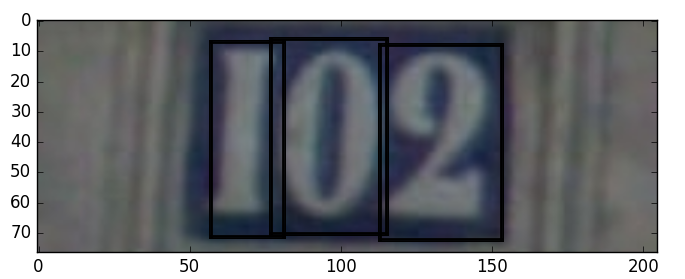
\includegraphics[width=0.9\linewidth]{images/figure_og.png}}
\end{center}
   \caption{An example image from the Training dataset. Bounding boxes for each
   			digit has been added to the image.}
\label{fig:Original Figure}
\end{figure}

Figure \ref{fig:6 Digit Figure} contains an example of an image that could be considered an outlier. 
This is the only digit in the Training set that contains a sequence of length 
six. This is not removed from the dataset however because in real world use of 
this network capturing sequences that include more than five digits seems fairly 
common. In the case of a mapping application that is trying to find addresses 
that are up to length five it is important to be able to find sequences that are 
longer than five digits and disregard them rather than creating two outputs that 
overlap or some other unexpected prediction.

%% 6 digit picture %%
\begin{figure}[t]
\begin{center}
\fbox{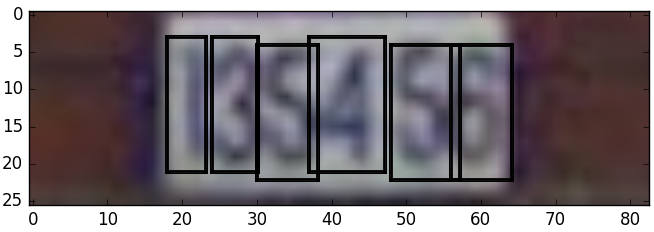
\includegraphics[width=0.9\linewidth]{images/6_digits.png}}
\end{center}
   \caption{The only example in the training dataset that has six digits.}
\label{fig:6 Digit Figure}
\end{figure}

%-------------------------------------------------------------------------------
\subsection{Algorithms and Techniques}

The following algorithms will be used to implement a deep convolutional neural 
network to identify multidigit sequences in real world scenes.
\begin{itemize}
	\item Logistic Regression: Using a matrix and a vector you can transform an 
	input of size $i$ into an output of size $o$ by multiplying the input by an 
	$[i, o]$ matrix then adding a vector of size $o$ to it. By adjusting the 
	value of the matrix an output can be created that depends on different parts
	of the input with different weights based on the matrix. Logistic Regression 
	is the defacto standard for neural networks which is why it is used here.
	\item Rectified Linear Unit (ReLU) Activation: Rectifier activation is used 
	to introduce non-linearity to the network. When passed through a ReLU 
	rectifier input is set to zero when below a threshold (the default 
	tensorflow threshold is used). ReLU is used because it causes sparse 
	activation (only some of the inputs are active) and it is efficient to 
	compute.
	\item Convolution: Using a small matrix called a kernel that is size x by x 
	by depth of the input (depth1) by depth of output (depth2) the kernel is moved
	over the input (the amount the kernel is moved is called the stride) 
	that is of depth1 and transforms the input into an output 
	that is slightly smaller but is now depth2. There are two forms of padding 
	that can be done, valid padding where the kernel never leaves the image and 
	same padding where the image is padded with zeros. This is a form of weight sharing 
	where the same weights are applied to various parts of the image so that the 
	network does not have to deal with where in the input the important features 
	are. As the kernel moves across the image it preforms logistic regression on 
	each piece of the input.
	\item Max Pooling: Small sections of the image are grouped together and the 
	largest value is used. This reduces the size of the input while retaining the
	depth of the input. Max pooling was chosen because it was used in AlexNet ~\cite{alex}, 
	which was a large influence on this network.
	\item Local Response Normalization: This restricts the values that are 
	possible to a smaller range while still having the relative ratios between 
	values in the input. This restriction helps reduce overfitting in the model 
	where the model is tuned so well to the training data that it fails to 
	generalize to the test data. This overfitting manifests as a low training 
	error and a high test error. Default parameters from tensorflow are used.
	Local response normalization was chosen, like max pooling, due to it's use 
	in AlexNet ~\cite{alex}.
	\item Dropout: When applied to an input layer it randomly zeros out some 
	values according to some probability. The fact that any given input may not 
	be present means that the network cannot depend on any one input feature. 
	This forces the system to learn redundant representations which leads to 
	more general solutions. Dropout was shown to be helpful by Goodfellow \etal 
	in their paper ~\cite{goodfellow}.
	\item Softmax: Softmax is an algorithm that normalizes the output values of 
	logistic regression. This makes it so the output sums to one and is a valid 
	probability distribution that can be used to make predictions. Softmax is a 
	classic algorithm used in image recognition to turn the results of logistic 
	regression into a probability distribution and so it is used here.
	\item Cross Entropy: Cross entropy is a metric that is used to tell how wrong 
	a prediction is compared to the correct answer. This loss function summarizes 
	how wrong the the model was when comparing its predictions to the real answers.
	It is the cost function that is used in logistic regression and is therefore 
	used here.
	\item AdagradOptimizer: Is an advanced optimization function that is 
	implemented in tensorflow that takes as inputs the gradients (partial 
	derivatives in respect to each weight variable) of the cost function and 
	updates these weights. This is an efficient and built into tensorflow so it 
	is a good choice to use.

\end{itemize}

The deep convolutional neural network is built with four convolutional layers 
that will transform the input which is size 50 by 50 by 1 (a grayscaled image) into a single feature 
vector of length 128. This feature vector will be passed to six logistic regression 
classifiers that each have hidden layers. These six classifiers will output the 
length and the values of the digits in the images. This network will work directly 
on the pixel values of the input images

\begin{enumerate}
	\item The first convolutional layer uses a kernel of size 3 by 3 by 1 by 16 
	and a stride of 1. The layer uses valid padding. This convolution reduces the 
	size of the image from size 50 by 50 by 1 to 48 by 48 by 16. Then max pooling is 
	applied to the input with a stride of two. This results in an image that is 
	size 24 by 24 by 16. This pooling is followed by local response normalization 
	to help reduce overfitting.
	\item The second convolutional layer uses a kernel of 1 by 1 by 16 by 32 and 
	a stride of 1. This means that the result of the convolution is the same size 
	as the input but it is much deeper (32 compared to 16). This technique of a 
	convolutional layer that does not reduce the input size but increases the 
	depth is taken from the implementation of a similar network by Goodfellow 
	\etal ~\cite{goodfellow}. After this second convolution local response 
	normalization is applied again. Changing this order of pooling and 
	normalization is adapted from the AlexNet architecture used by Krizhevsky 
	\etal to win the ImageNet competition in 2012 ~\cite{alex}. Then pooling is 
	applied resulting in an input of 12 by 12 by 32.
	\item The third convolution is then applied with a kernel of size 5 by 5 by 
	32 by 64 and a stride of 1 to create an output with size 8 by 8 by 64. 
	Pooling is used to change the size to 4 by 4 by 64. Normalization is then 
	applied.
	\item The final convolution with kernel 1 by 1 by 64 by 128 and stride 1 is 
	then applied to create a input of 1 by 1 by 128. This input is normalized 
	and then reshaped into a feature vector of size 128.
\end{enumerate}
 
This final feature vector is then used as input for six different softmax classifiers that 
have hidden layers of size 16. The first softmax classifier has an output space 
of 0 to 6 (the length of the sequence in the image) and the rest have output 
spaces of 0 through 10 (the values of the digits in the image). These softmax 
classifiers show the probability that a certain digit is that value.by taking 
the most probable value we can make predictions of the digits in the image. In 
this network dropout is applied to each layer save input and output. 

The results are compared to the labels using 
``sparse\_softmax\_cross\_entropy\_with\_logits'' to calculate the loss. This 
cost is then minimized by the AdagradOptimizer in order to train the model.

%-------------------------------------------------------------------------------
\subsection{Benchmark}
According to the paper by Goodfellow \etal ~\cite{goodfellow} human operators have about 98\% 
accuracy when it comes to identifying multidigit sequences in natural scenes. 
This would obviously be a good benchmark to try to reach with this system. 
However the system created by Goodfellow \etal ~\cite{goodfellow} only reached 96\% accuracy in natural scenes. 
This state of the art result seems to be a better benchmark than humans levels 
(it seems more obtainable that trying to beat state of the art results). However
this result seems unobtainable due to the development environment. Goodfellow 
\etal ~\cite{goodfellow} achieved 96\% using a neural network that was eleven layers deep before 
being connected to the six final output layers. The final feature vector created by
Goodfellow \etal's convolutional network was of size 4096 while the vector created 
by this convolutional network is only of size 128 ~\cite{goodfellow}. Goodfellow \etal ~\cite{goodfellow}used a 
distributed framework called DistBelief to train their network and it still took 
six days to train the network. Time and resources to create such a deep network 
are lacking. Using a shallower network (about four or five layers) should be able to
reach about 90\% accuracy according to the graph in Figure 4 of the Goodfellow 
\etal paper ~\cite{goodfellow}. 

Due to the large amount of samples that have a small length of sequence a poor model 
might be tempted to guess all 10 (the ``not there value''). If the model also 
guessed all the sequences were length 2 (the mode of the training set) then this 
model would achieve an accuracy of 60.79\%. This sets a floor that the model 
should try to beat.

%%%%%%%%%%%%%%%%%%%%%%%%%%%%%%%%%%%%%%%%%%%%%%%%%%%%%%%%%%%%%%%%%%%%%%%%%%%%%%%%
\section{Methodology}
%-------------------------------------------------------------------------------
\subsection{Data Processing}

Data processing for this problem was based on the processing methods described
by Goodfellow \etal in their paper ~\cite{goodfellow}. First a bounding box that encompasses 
all the bounding boxes for the digits in the images is found. This box is not included
in the labels from the dataset. It is instead programmatically found by finding 
the highest, lowest, leftmost, and rightmost parts of the provided bounding boxes 
(the one that surround each digit) and creating a box of that size. This box is then 
scaled up by 30\%. The image is then cropped to the size of this scaled up box.
This cropped image is then resized to be 50 pixels by 50 pixels. In the paper
by Goodfellow \etal ~\cite{goodfellow} these images are resized to 64 pixels by 64 pixels. This
was the first size tried but the development environment ran out of memory
when they were scaled to 64 pixels by 64 pixels, after trying several sizes 50
seemed to be the largest that my development environment could handle. After the 
resizing the images were converted from the RBG with 3 color channels to grayscale 
so that rather than three channels the resulting images had only one color channel. 
Finally the images are normalized by subtracting the mean pixel value from each 
pixel and dividing it by the standard deviation. This regularization was the 
only form applied to the dataset. Things like LeCun Local Contrast Normalization 
were not used.

As explained above the one image with length six could be considered an outlier 
but was not removed from dataset due to high likelyhood of similar images being 
found in the wild 

The SVHN dataset is divided into three datasets. The train, test, and extra datasets.
The extra dataset is a large collection of easy samples while the train dataset is 
a smaller dataset with ``more difficult'' samples. The difficultly assessment for 
these datasets comes from both a paper by LeCun \etal ~\cite{sermanet-icpr-12} and 
the sentiment is echoed by the website where the dataset can be downloaded. To create 
training and validation datasets from the train and extra datasets a method from LeCun \etal ~\cite{sermanet-icpr-12}
was used. The Validation set is created so that it is $\frac{2}{3}$ train samples 
and $\frac{1}{3}$ extra samples from each class. This breaks down into about 4,000 
train samples of each class and about 2,000 extra samples from each class 
(5684 total). Here ``class'' is defined to be based on what digit is the first 
in the sequence in the image.

Figure \ref{fig:Processed Figure} shows Figure \ref{fig:Original Figure} after the image has been processed.

%% Processed figure %%
\begin{figure}[t]
\begin{center}
\fbox{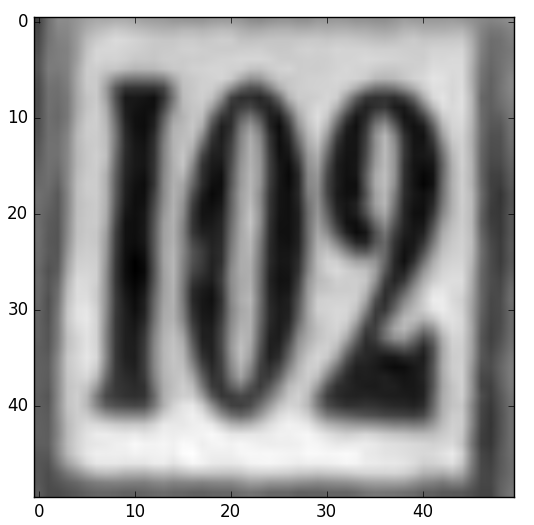
\includegraphics[width=0.9\linewidth]{images/figure_processed.png}}
\end{center}
   \caption{The same image from Figure 1 after it has been processed (cropped, 
   			resized to 50 x 50 pixels and converted to grayscale). }
\label{fig:Processed Figure}
\end{figure}

%-------------------------------------------------------------------------------
\subsection{Implementation}
The first step in implementation was to obtain the datasets. These were fetched 
from \url{http://ufldl.stanford.edu/housenumbers/} using a modified version of 
the download code from the deep learning course at Udacity 
\url{https://www.udacity.com/course/deep-learning--ud730}. The code can be found here
\url{https://github.com/tensorflow/tensorflow/tree/master/tensorflow/examples/udacity} The data was then 
extracted using more code modified from the deep learning course. 

While implementing the data preprocessing familiarity with numpy was needed to help 
shape and normalize image arrays. The very tricky part came from the format of 
the SVHN label file. The labels were saved as a .m matlab file. With the newest 
versions of matlab python cannot turn the data from a .m file into a dictionary 
automatically. 

The use of the h5py module was new during this project. h5py was used to read 
data from the .m file and parse it into python dictionaries. This was one of the 
trickier parts of the project and help from the Udacity forms really helped get 
a handle on the way that h5py uses references and how to fetch data from it. The 
code used is adapted from \url{https://github.com/hangyao/street_view_house_numbers/blob/master/3_preprocess_multi.ipynb}

Once the preprocessing code was written the next problem that was ran into is the
limitations of the development environment. This was all done on a laptop and when the 
preprocessing code tried to resize all images to be 64 by 64 pixels the program 
would run out of memory. This meant that a new size must be found. After trying 
smaller and smaller resize dimensions 50 seemed to be the largest dimensions that 
the images can be scaled down to without running out of memory.

The Neural Network itself was implemented in tensorflow by Google ~\cite{Google} 
This was the first time using tensorflow but it was fairly easy. First it was 
implemented as a straight block of code in an ipython notebook. This was 
obviously non-conducive to using in an application. The network was rewritten 
using functions. This took a long time to figure out how to do because of 
inexperience with tensorflow, especially the fact that things are not evaluated 
until a session is run, plus the idea of a graph and how to use placeholders 
took a bit to get used to. This code still looked unreadable so variable scope 
was added to clean it up. Tensorboard summary operations were also added to help 
visualize both the model and the learning process. Figure \ref{fig:model image} shows the visualization 
of the entire tensorflow graph. Figure \ref{fig:network figure} shows the graph of actual network itself.


%% Model picture %%
\begin{figure}[t]
\begin{center}
\fbox{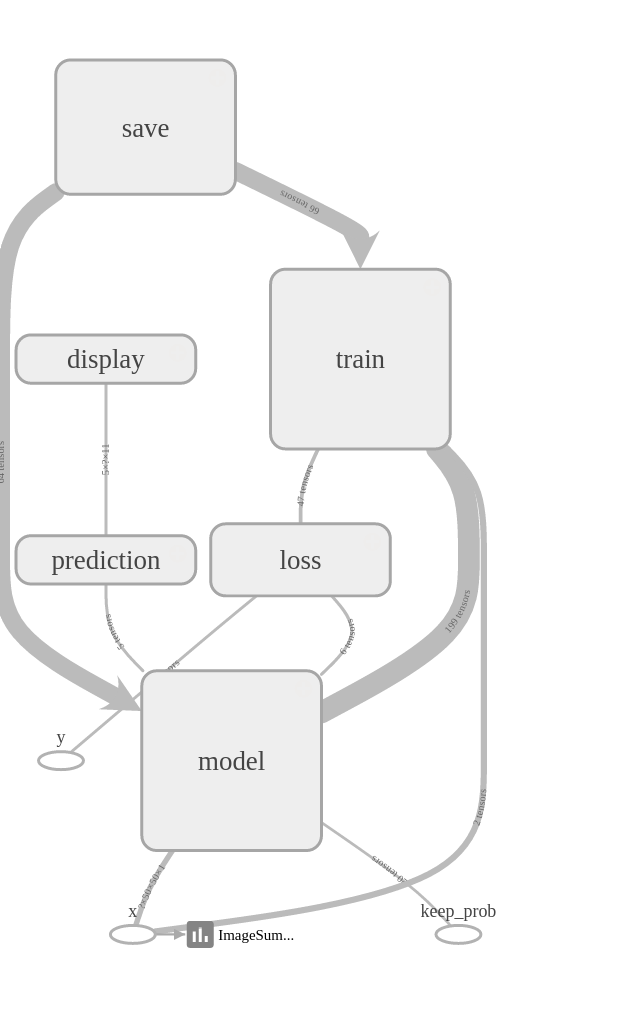
\includegraphics[width=0.5\linewidth]{images/model_graph.png}}
\end{center}
   \caption{A picture of the tensorflow graph. The model is the network itself 
   and the rest of it is the what allows for training and saving the graph.}
\label{fig:model image}
\end{figure}

%% Network picture %%
\begin{figure*}
\begin{center}
\fbox{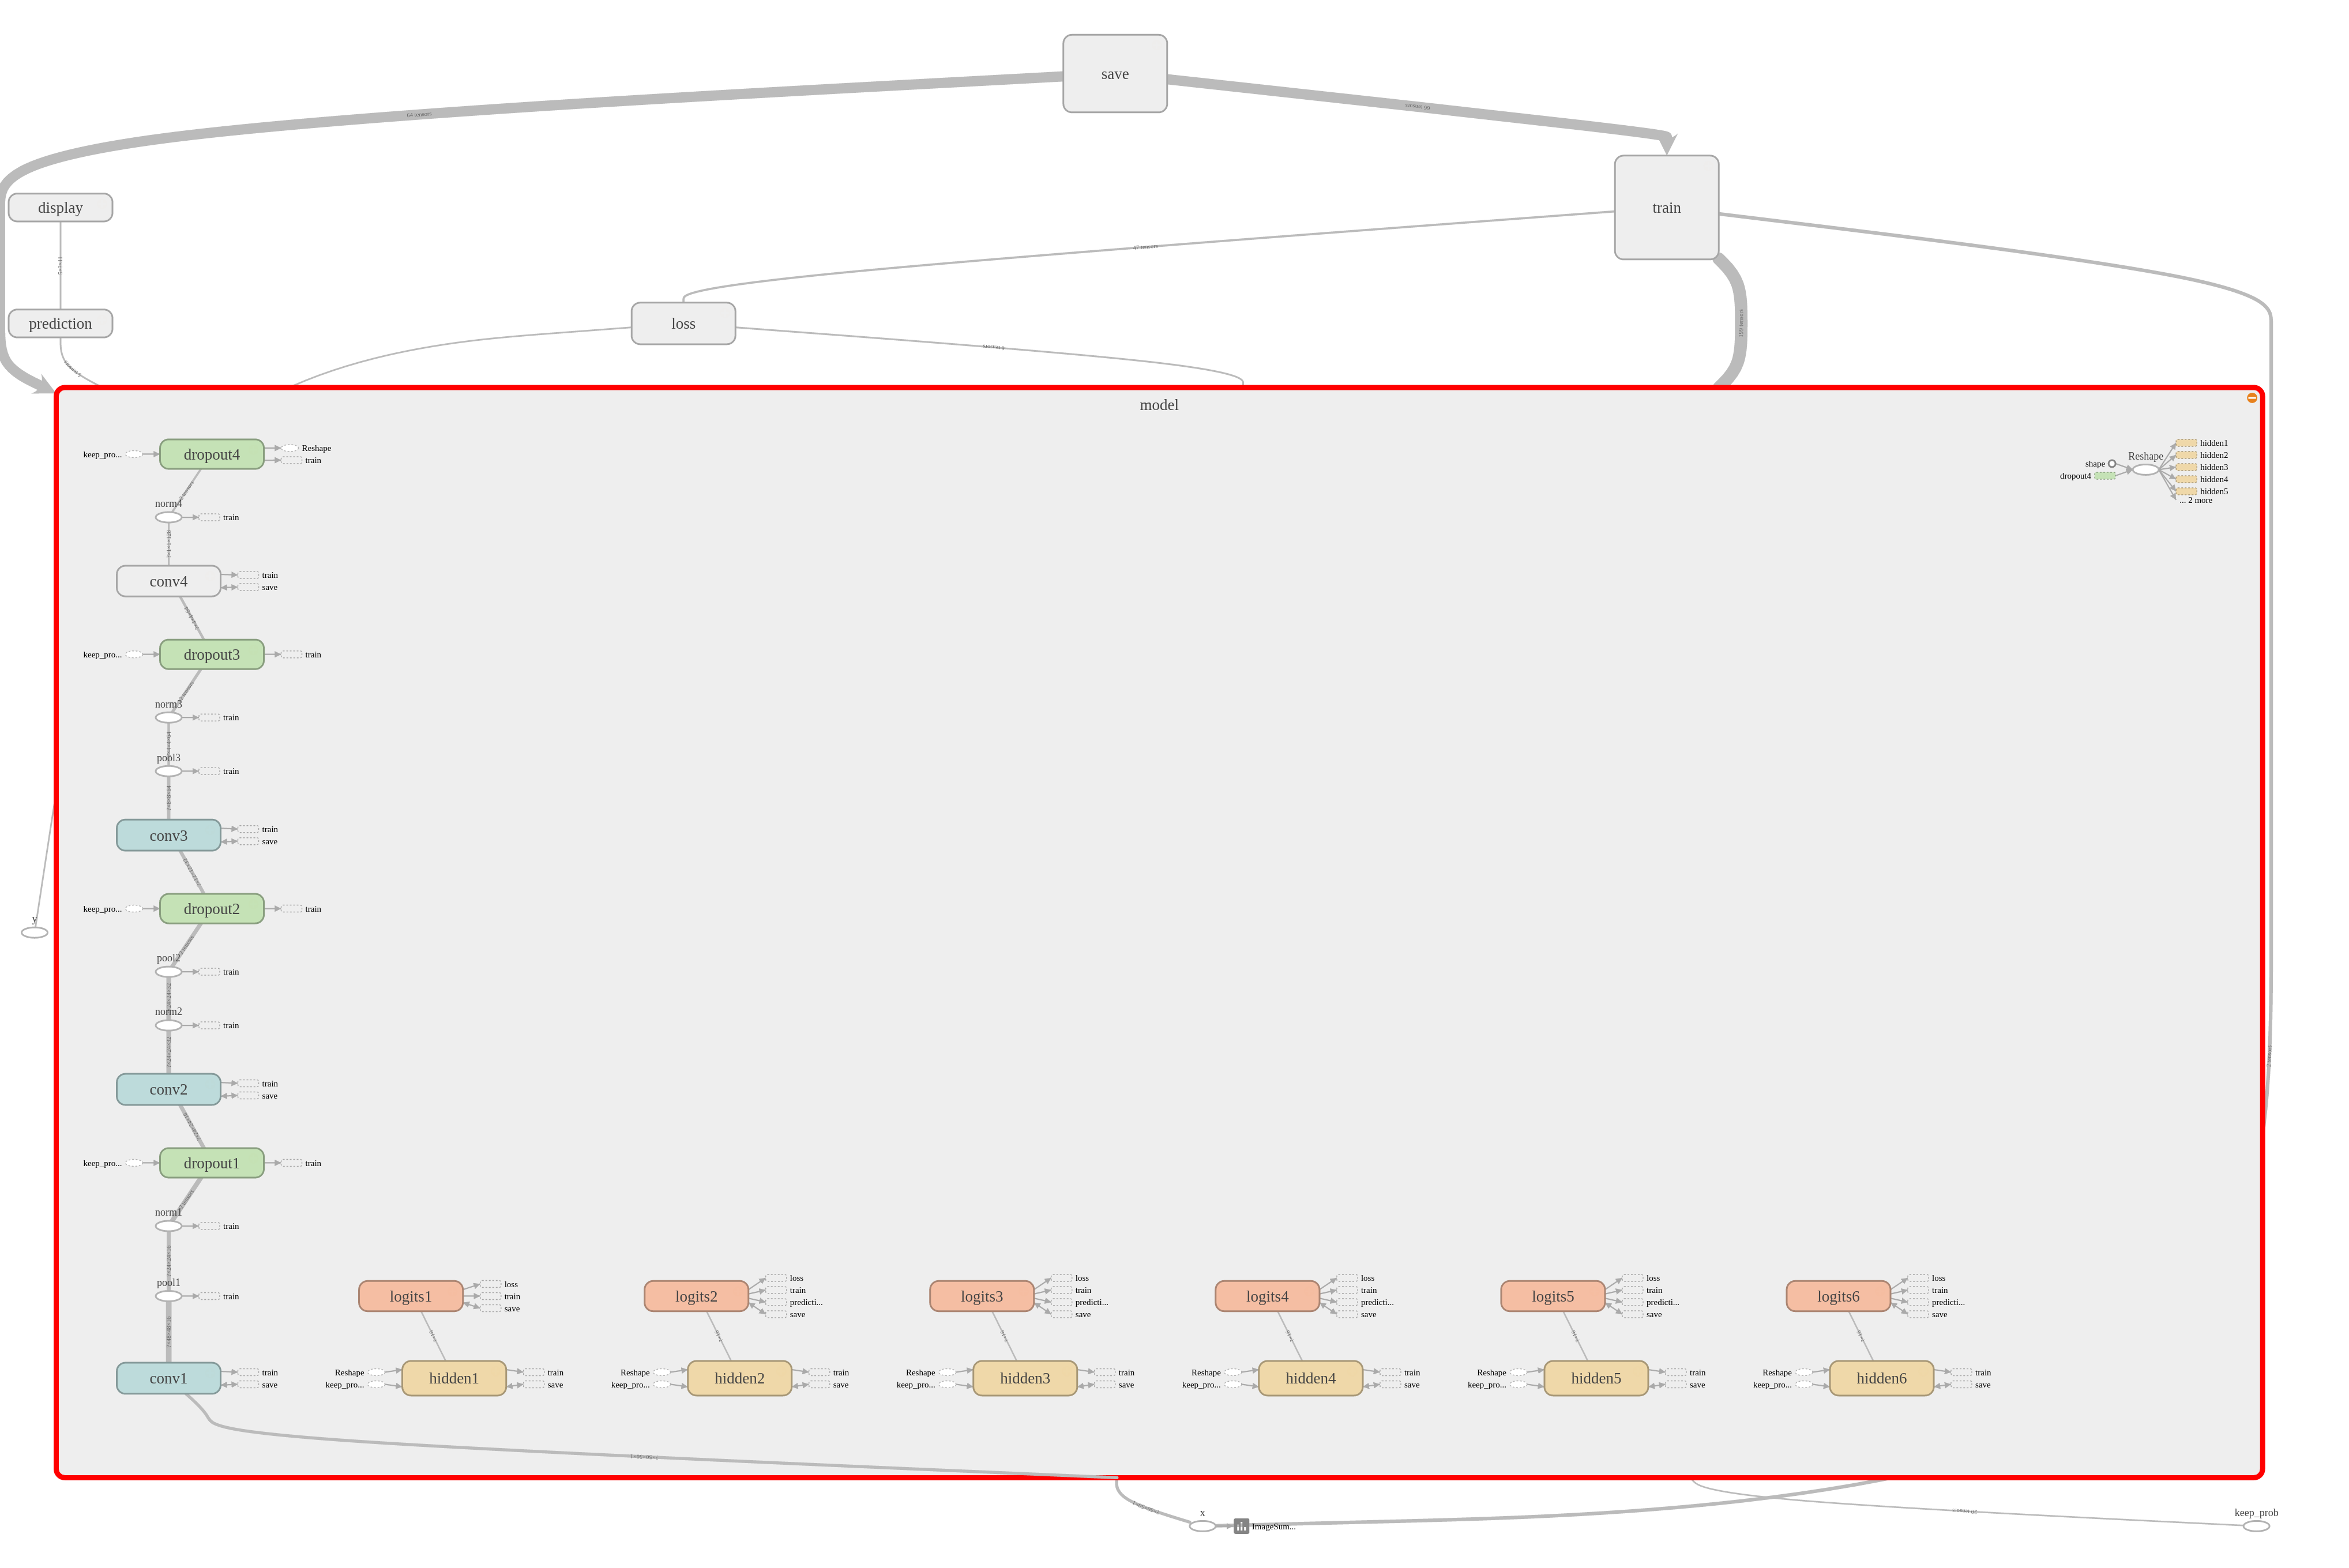
\includegraphics[width=0.9\linewidth]{images/network_graph.png}}
\end{center}
   \caption{Picture of the network from tensorboard. 
   Larger image avaiable at \url{http://imgur.com/cx9DINa}}
\label{fig:network figure}
\end{figure*}

The trickiest part of the implementation was how to calculate the loss function 
for this network. Most softmax implementations use cross entropy with the 
label ``one-hot encoded'' (the label is a vector that has a 1 in the index of the 
answer rather than just being a scalar that is the answer). Not wanting to 
convert labels into ``one-hot encoded'' labels ``sparse\_softmax\_cross\_entropy\_with\_logits'', 
the tensorflow function that calculates the cross entropy, was used. The use of 
this function meant that cross entropy could be calculated  
without needing to use ``one-hot encoded'' labels (which would have been a drain 
on system resources). The tensorflow documentation 
mentions that input to this function should be the output of logistic regression 
rather than output of softmax because the function does softmax itself to be more 
efficient. This required a slight rewrite as the inference function that builds 
network graph originally returned the softmax of the logits layer. The function 
needed to return the logits layer instead so that it could be used with the 
``sparse\_softmax\_cross\_entropy\_with\_logits'' function. To calculate the 
actual loss the result of ``sparse\_softmax\_cross\_entropy\_with\_logits'' had 
to be summed for each label compared to each logits output layer. That is each 
of the six logits outputs a prediction and the 
``sparse\_softmax\_cross\_entropy\_with\_logits'' was used to find the cross 
entropy between each of the logits output and the label that corresponds to that 
logits. These results where then summed up. 

%% Loss graph %%
\begin{figure}[t]
\begin{center}
\fbox{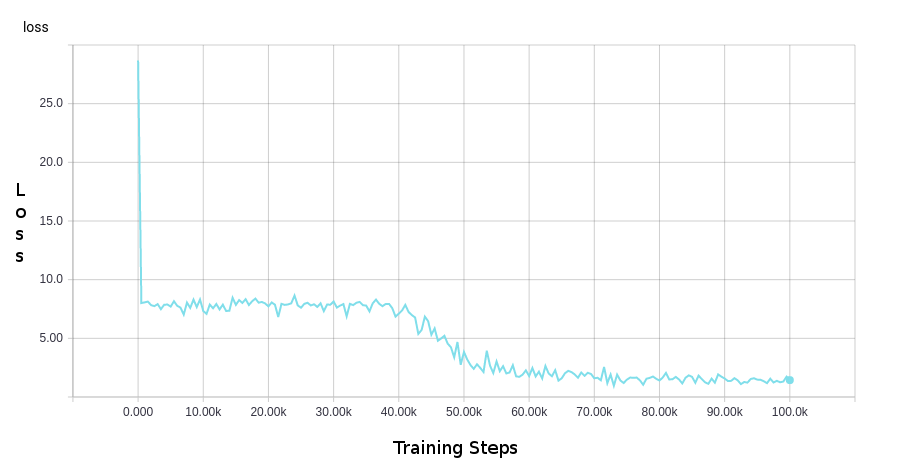
\includegraphics[width=0.9\linewidth]{images/loss_graph.png}}
\end{center}
   \caption{This graph of the loss function over training steps shows how the loss
   decreased as the model was trained.}
\label{fig:loss}
\end{figure} 

Figure \ref{fig:loss} shows 
the change in the loss function at various training steps. The loss function 
trended down during training showing that it is a good loss function and minimizing 
it helped train the model. 
%-------------------------------------------------------------------------------
\subsection{Refinement}
The original model had only three convolutional layers and no hidden layers in 
the logits. It also only had dropout between the final feature vector and the 
logits layers. This model had the accuracy reported in the first row of 
Table \ref{table:acc}. While the test accuracy is reported in this table it was not used to 
tune the model as this would cause the features of the test set to bleed into 
the training process. The fact that the the training and validation accuracy is 
low means that the model is not complex enough to represent the data (the model 
has high bias). Due to these errors the network was made deeper, another 
convolutional layer was added, and larger, hidden layers were added to the 
logits. 

Once the network was expanded the accuracies were the ones found in the 
second row of Table \ref{table:acc}. The fact that the validation error is so much higher than 
the test set error (shown by the fact the the accuracy is lower) means that the
model is overfitting to the training data. The model has high variance and is having 
trouble generalizing to the test data and will likely have trouble on other novel 
data. A common technique to fight overfitting in neural networks is dropout. This 
was then added to each layer of the model outside of the input and output layers.

Once the network was made larger and dropout was added the accuracy reported in 
row 3 of Table \ref{table:acc} were found. Similar steps (especially increases in depth) could 
be taken from here to get even better performance.
%-------------------------------------------------------------------------------
\section{Results}
\subsection{Model Evaluation and Validation}

The final model is a deep convolutional neural network. This model was chosen due 
to its use by Goodfellow at all ~\cite{goodfellow} to great success. The final 
model however was deeper than the original plan for the model. This more complex
model resulted in very long training times, 11.18 hours on an Intel i5 CPU.

Figure \ref{fig:accuracy} shows the accuracy values for the training and validation 
datasets as training went on. The validation set was still increasing as the training
went on meaning that more training could increase the accuracy. Table \ref{table:acc}
includes the final Test accuracy of 93.89\%. This accuracy is close to the 
training and validation accuracy which means that this model does not suffer from 
high variance. The means that the model does not overfit to the training data and 
is able to generalize to new data. This model is therefore a good fit to solve 
this problem.

In addition to using the Test set to test the model's performance, the performance was vetted using 
both a camera application and the ability to run the model on various images. The 
model preforms reasonably well on these applications. However when these input 
methods have a slight problem in that they preform rather poor when the digits 
are not centered in the image. Unlike Test set images these Camera images do not 
have bounding boxes and therefor don't have a way to center the images. 
They also preform better when the digits are about
30\% smaller than the boundaries of the images. These input methods show that the 
model is sensitive to slight changes in the input. This could be fixed with a 
deeper network and more input where the digits are in various places of the input.
This problem could also be solved with more convolutional layers because 
convolutions squeeze the spacial dimensions from the images. Without having the 
digits in various places in the input images the model never really learns to 
localize the digits.

%% Accuracy Graph %%
\begin{figure}[t]
\begin{center}
\fbox{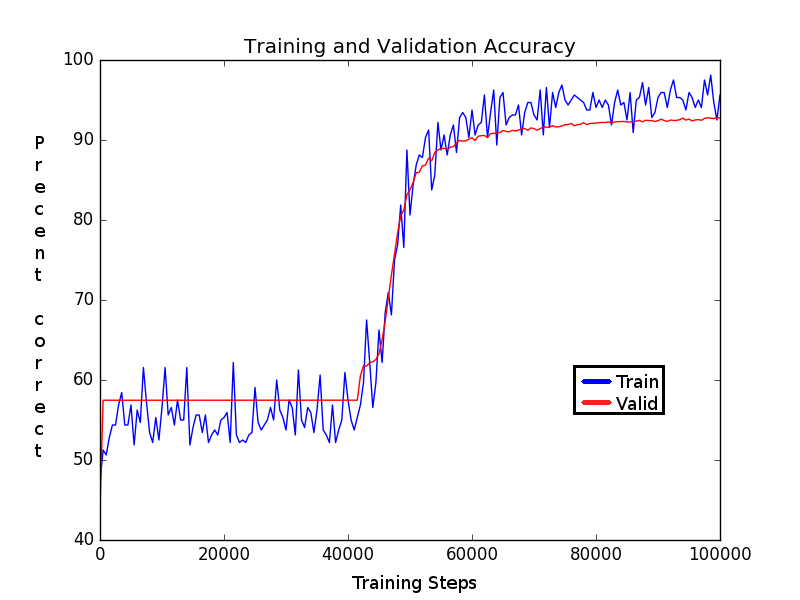
\includegraphics[width=0.9\linewidth]{images/accuracy.png}}
\end{center}
   \caption{A graph showing how the accuracy on the training batch and the 
   accuracy on the validation set changed as the model was trained.}
\label{fig:accuracy}
\end{figure}

%% Accuracy Table %%
\begin{table}
\begin{center}
\begin{tabular}{|l|c|c|c|}
\hline
Accuracy & Train & Valid & Test \\
\hline
Original & 90.13 & 88.38 & 89.45 \\
\hline
Second & 95.21 & 90.39 & 91.11 \\
\hline
Best & 95.63 & 92.73 & 93.89 \\
\hline
\end{tabular}
\end{center}
\caption{Accuracy of the model on each dataset where the Train dataset is the
last accuracy on the last batch of training data.}
\label{table:acc}
\end{table}

The results of this model is quite strong and can be trusted in applications where
wrong answers are not the worst thing in the world. If the network was being used 
for mapping data where a wrong address could mean sending a user to the wrong place 
then the model would have to be trained more.

Currently only one validation set is used to validate the model. Normally cross-validation 
is used to create multiple validation sets which are used to validate the model. This 
insures that there is not some hidden pattern in the validation set that is leading 
to abnormally high or abnormally low results. This was not done due to time 
constraints but will be done in the future when improvements are made to the model.

This model generates digits found in natural scenes. The model creates usable 
output and is a good solution to the problem.

%-------------------------------------------------------------------------------
\subsection{Justification}

%% Example output %%
\begin{figure}[t]
\begin{center}
\fbox{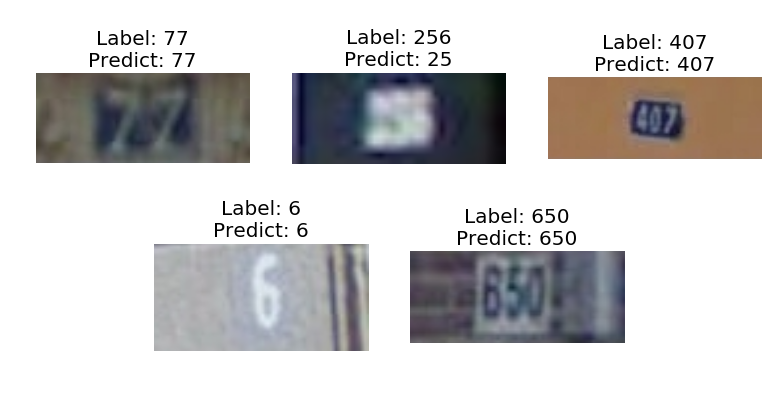
\includegraphics[width=0.9\linewidth]{images/example_output.png}}
\end{center}
   \caption{An example of some of the output of the model. The images are images
   that were fed into the model. The Label is the label for that image from the 
   dataset and the Predict is the value of the output when that image is feed into 
   the network.}
\label{fig:output}
\end{figure}

Figure \ref{fig:output} show several example outputs. It includes the image that 
was given to the network, the label from the dataset and the predicted digits 
in the image from the model. The model missed only a single digit from the second 
image. 

This model sufficiently solves the problem. A network that guessed only 2 for the 
sequence length and only 10 for the each digit would score 60.79\%. This is the 
minimum accuracy required for the system to do better than educated guesses. The
test accuracy for the final network is 93.89\%. This is far better than the 
minimum benchmark. 93.89\% is also pretty close to the accuracy found by Goodfellow
\etal ~\cite{goodfellow}. Being close to this benchmark is a very good result.

This network is a good solution to the problem. It has a few selectivity problems 
as discussed in the ``Model evaluation and validation'' section. When the 
improvements mentioned later in the ``Improvements'' section are applied then 
these problems may disappear. Even before these improvements the model does a 
good job classifying digits.

%-------------------------------------------------------------------------------
\section{Conclusion}
\subsection{Free Form Visualization}
While there is not much more to visualize as the dataset is just images so most 
of these visualizations will be about the learning process.

Figure \ref{fig:two image} shows two images. The left is a processed image that has been resized 
and converted to grayscale. The right side of the photo is the image after it 
has passed through one convolutional layer. The changes to the image show how the 
convolution change the image. It is hard to see the reduced size because it is 
only two pixels smaller.

%% Two image pictures %%
\begin{figure}[t]
\begin{center}
\fbox{
	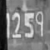
\includegraphics[width=0.5\linewidth]{images/input_image.png}
	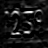
\includegraphics[width=0.5\linewidth]{images/conv_image.png}
}
\end{center}
   \caption{The image on the left is one of the images that has been processed 
   and is ready to be fed into the network. The image on the right is the image
   after it has been through a single convolution.}
\label{fig:two image}
\end{figure}

The following Figures, \ref{fig:conv}, \ref{fig:hidden}, and \ref{fig:logits}
are histogram activations for various 
weights in the convolutional network. Figure \ref{fig:conv} shows the activation for the 
weights in the third convolutional layer of the network. Figure \ref{fig:hidden} shows the 
histogram activation for the hidden layer in the 5th logits layer. Figure \ref{fig:logits} 
shows the activation for one of the final logits layer. 

%% Convolutional graph %%S
\begin{figure}[t]
\begin{center}
\fbox{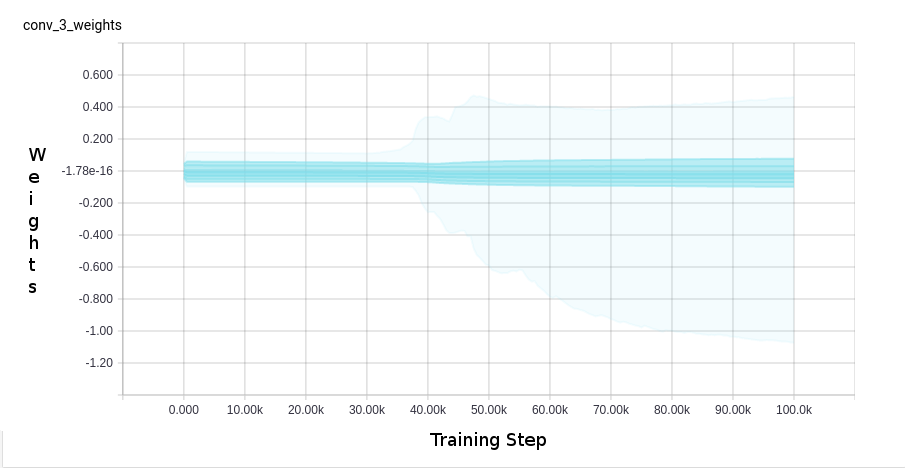
\includegraphics[width=0.9\linewidth]{images/conv_3_graph.png}}
\end{center}
   \caption{This shows the activation of the third convolutional layer weights in 
   the network. The top and bottom light blue lines show that the training doesn't 
   begin to effect this set of weights until almost 40,000 training steps.}
\label{fig:conv}
\end{figure}

%% Hidden Graph %%
\begin{figure}[t]
\begin{center}
\fbox{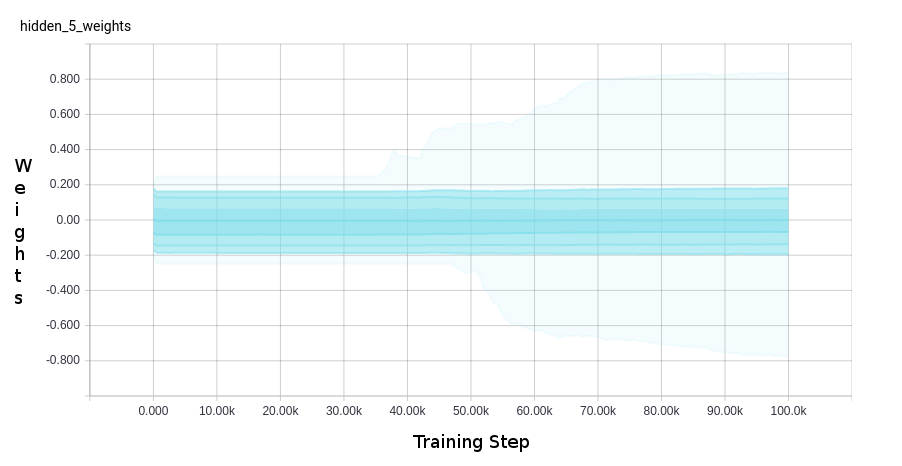
\includegraphics[width=0.9\linewidth]{images/hidden_5_graph.png}}
\end{center}
   \caption{This shows the activation of the hidden layer weights in the fifth logits in 
   the network. The top and bottom light blue lines show that the training doesn't 
   begin to effect this set of weights until almost 30,000 training steps.}
\label{fig:hidden}
\end{figure}

%% Logits Graph %%
\begin{figure}[t]
\begin{center}
\fbox{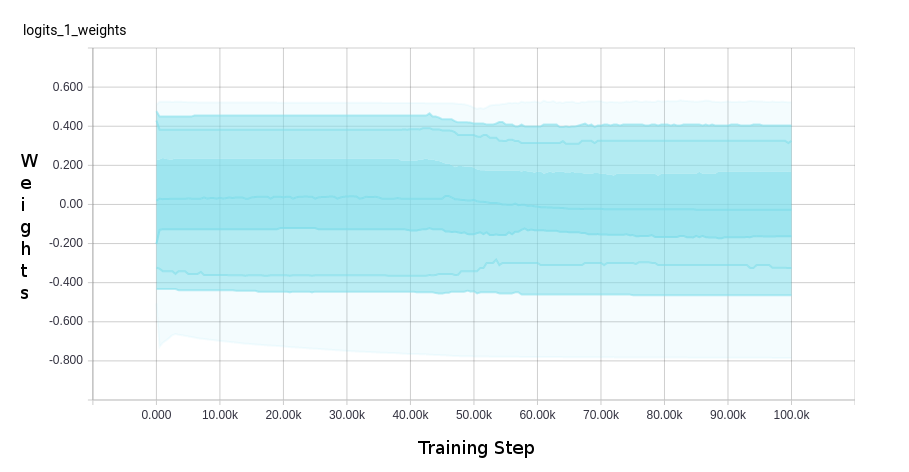
\includegraphics[width=0.9\linewidth]{images/logits_1_graph.png}}
\end{center}
   \caption{This shows the activation of the output layer weights in the first logits in 
   the network. The top and bottom light blue lines show that the training starts to change 
   weights almost immediately.}
\label{fig:logits}
\end{figure}

These graphs are a little hard to read but they show the distribution of the 
activation on each layer. The middle line is line that splits the activations so 
that 50\% fall above it and 50\% below. The dark lines are the lines where 69\% 
of the activations fall between them, while the light blue lines are where 89\% 
fall between. All three of these graphs show what the majority of activations 
(between the blue lines) are. The differences between the graph shows how the 
different layers are trained. The deepest layer (convolution 3 weights in Figure
\ref{fig:conv}) is the slowest to change. This change is visible due to the expansion in the 
y dimension of the top and bottom lines in the graph. The hidden layer changes 
quicker and the logits changes the quickest in that it already starts with a 
wide distribution and stays wide. The explanation for the difference between 
these graphs is explained by the saturation of the logistic function at different 
levels of the neural network ~\cite{xavier}. These graphs help visualize the learning process and 
in future runs and improvements these graphs will help see patterns and show that
the changes are helping the models performance.

%-------------------------------------------------------------------------------
\subsection{Reflection}

The first step of this project was to read the existing literature available on 
the topic. The most helpful papers were by Goodfellow \etal ~\cite{goodfellow} and 
LeCun \etal 
\cite{sermanet-icpr-12}. The Goodfellow \etal ~\cite{goodfellow} paper was especially helpful. That 
is where the idea of creating a single convolutional feature vector and using 
that as input to various logitic classifiers.

The next step was to analyze and process the dataset. This was an interesting part 
of the process because the use of h5py was new and without this project it would
probably not have been used. The h5py module is used to access data structures 
that are saved on to disk.

After processing the data the model was build in tensorflow. This was an 
interesting part to the project be cause it was new. Figuring out how to build 
the convolutional network so that the final feature vector was only size 1 by 1 
by depth. The difficult part was turning the mess of spaghetti code into a well 
organized function, several errors were introduced in the process that resulted 
in very low accuracy (the cross entropy error did take into account the 4th 
logits). Figuring out the cause of this error took several days and was the 
hardest part of the project.

The final steps was adding the network into an application. This was interesting 
to use opencv for the first time. After hooking all the pieces together the last
thing to do was train the model. This took 11 hours and the anticipation was one 
of the harder parts of the project.

This is one of the largest end-to-end projects that have been undertaken and while 
the results are a little weaker than the goal was, the project was a large success.
%-------------------------------------------------------------------------------
\subsection{Improvement}
There is a lot of improvement that can be made from here. One of the first things 
that might be able to help performance would be to normalize the data after it 
is split into the training and validation set rather than before. This would help 
make the images within a dataset more uniform.

Another problem that the model has is that it struggles when the digit sequence 
is not in the center of the image. This problem, plus the problem that the 
accuracy is not as high as it could be, can be solved in a single tweak. As 
discussed in the paper by Goodfellow \etal ~\cite{goodfellow} more data can be artificially created 
by grabbing different parts of the bounding box. For example once you blow up the
largest bounding box you can grab the whole thing as one data point, you can grab 
top left box (from the scaled up corner top left to the original bottom right 
corner) so the image is in the lower right part of the image and so on. This means that a single
image can be used to create 5 training points. This would help train the model to 
detect digits where ever they appear in the image. The increase in amount of data 
will also help the accuracy of the model. 

In order to do some of the other improvements a better development environment 
is needed. One obvious improvement is during data preprocessing resize the images 
to 64 by 64 rather than 50 by 50. This allows for more pixels and clearer images. 
This will help performance but requires more memory for the computer.

As the Figure \ref{fig:loss} loss function graph shows that at the end of the training steps 
the loss function was still decreasing. The same trend is shown in Figure \ref{fig:accuracy} as 
the accuracy continues to increase. This means that the model would benefit from
more training. The training time for the best model was 11 hours long so in order 
to realistically train for significantly more steps would require a GPU to speed 
up training and allow for more training.

Another improvement is to create a more complex model. This means a deeper 
convolutional network and more hidden units in the logits layers as well as more 
hidden layers. This also can mean using larger convolutional kernels and same 
padding. A more complex network also means that it is possible to over fit so 
dropout is needed. For this deeper network to be feasible parallel training on a 
GPU would be needed for training. The largest indicator that the deeper network 
would help is the fact that the Goodfellow \etal ~\cite{goodfellow} paper had a 
feature vector produced by the convolutional part of the network had a 4096 
features compared to the 128 features in this model.

The majority of improvements to this network boils down to having a large network 
and more data. This requires an improved development environment. This work 
should be easy to expand on and will be soon. 

{\small
\bibliographystyle{ieee}
\bibliography{bib}
}

\end{document}